\input sys/inputs.tex

\begin{document}

\bigheading{Vymedzené udalosti}

% \info{task_name}{infile}{outfile}{points}{timelimit}{memlimit}
% leave this values, if you are not interested
\info{critical}{stdin}{stdout}{100}{600 ms}{1 GB}

Žaba sa pri príležitosti svojich 21. narodenín rozhodol,
že už nebude tráviť svoj drahocenný čas nad exaktnými vedami
a stane sa historikom.

Hneď pri svojom prvom projekte však narazil na problém.
Skúmal $N$ historických udalostí
a potreboval určiť ich poradie.
K dispozícii mal $M$ dokumentov,
pričom každý z nich hovoril o práve dvoch udalostiach $u$ a $v$
a ich poradí.
Hovoríme, že udalosť $u$ bola skôr ako udalosť $v$,
vtedy, ak o tom hovorí niektorý z dokumentov,
alebo vtedy, ak existuje medziudalosť $z$ taká,
že $u$ bola skôr ako $z$ a zároveň $z$ bola skôr ako $v$.

Udalosť $u$ nazývame vymedzenou, ak pre každú inú udalosť $v$ platí,
že buď $u$ bola skôr ako $v$ alebo $v$ bola skôr ako $u$.
Môžete predpokladať, že Žabove dokumenty sú konzistentné
a teda o žiadnej udalosti nemôžeme povedať, že nastala sama pred sebou.

Žaba toto samozrejme vie nakódiť, ale je to hnusná exaktná činnosť
a tak to radšej nechá na vás. Nesklamte ho!

\heading{Úloha}
Napíšte program, ktorý pre dané dokumenty určí všetky vymedzené udalosti.

\heading{Vstup}
Prvý riadok obsahuje medzerou oddelené celé čísla $N$ and $M$.
$N$ ($1 \leq N \leq 100000$) je počet udalostí
a $M$ ($0 \leq M \leq 1000000$) je počet dokumentov.
Udalosti sú číslované od $1$ po $N$.
$i$-ty z nasledujúcich $M$ riadkov obsahuje
dve rôzne celé čísla $u$ a $v$ ($1 \leq u, v \leq N$)
hovoriace, že udalosť $u$ bola skôr ako $v$
podľa $i$-teho dokumentu.
\bigskip

V $40 \%$ prípadov navyše platí $N \leq 5000$ a $M \leq 30000$.

\heading{Výstup}
Na prvý riadok výstupu vypíšte jedno celé číslo, počet vymedzených udalostí.
Na druhý riadok vypíšte čísla vymedzených udalostí,
oddelené medzerami
a utriedené od najmenšieho po najväčšie.
Ak neexistuje žiadna vymedzená udalosť, druhý riadok nevypisujte.

\heading{Príklady}

\sampleIN
7 9
1 3
2 3
3 4
3 5
4 6
5 6
1 7
3 7
7 4
\sampleOUT
2
3 6
\sampleCOMMENT

\sampleEND

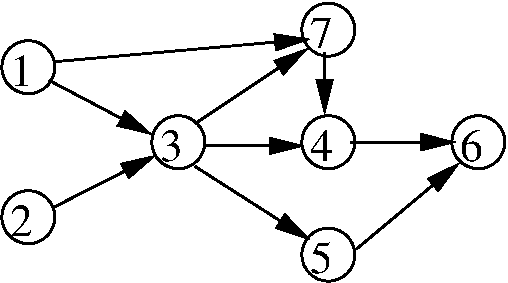
\includegraphics[height=4cm]{img/critical-fig.pdf}
\bigskip


\end{document}
